\setcounter{table}{0}
\renewcommand{\thetable}{S\arabic{table}}%
\setcounter{figure}{0}
\renewcommand{\thefigure}{S\arabic{figure}}%
\renewcommand{\thesection}{SI~\Alph{section}}%

\section{An external, spatially uniform potential $\V$ shifts the chemical potential $\mu$ of the gas} \label{sec:V_shifts_chem_pot}
We show that imposing an external, spatially uniform potential $\V$ to a gas
has the effect of shifting the chemical potential $\mu$ of the gas, recovering
eqn.~\ref{eq:mof-density}. Consider a control volume $\Omega$ with volume
$V=|\Omega|$ (large enough to neglect boundary effects) that is endowed with
the external, spatially uniform potential $\V$. Impose the grand-canonical
ensemble, where this control volume can exchange energy and particles with a
bath of gas at temperature $T$ and chemical potential $\mu$.

To denote a microstate of this system, let $N$ be the number of gas particles
in the control volume and $\mathbf{r}_1,...,\mathbf{r}_N$ be their positions.
Then, the potential energy $E$ of a microstate of the control volume is:

\begin{equation} E(\rvec_1,...,\rvec_N) = N\V +
E_{gg}(\rvec_1,...,\rvec_N),
\end{equation}
where $E_{gg}$ is the (unknown and complicated) interatomic potential for
gas-gas interactions that governs the (real) gas properties. The first term
arises from each gas molecule experiencing the external potential $\V$, where
$\V < 0$ corresponds to attraction. To account for molecular rotational and
vibrational degrees of freedom, we could treat the positions $\rvec_i$ as the
locations of atoms rather than molecules. In this case the gas-gas interactions
will include both \emph{intra-molecular} interactions and
\emph{inter-molecular} interactions.

The grand canonical partition function of the control volume is:

\begin{multline}
    \Xi(\mu, V, T)= \\ \displaystyle \sum_{N=0}^\infty \frac{1}{\Lambda^{3N}N!} \int_{\Omega} \cdots \int_{\Omega} e^{-\beta E_{gg}(\rvec_1, ..., \rvec_N)} e^{\beta (\mu - \V) N} d\rvec_1 \cdots d\rvec_N.
    \label{eq:gcpf}
\end{multline}
We recognize this as the grand canonical partition function of the bulk gas in
the control volume without the external potential, but shifted in chemical
potential:

\begin{equation}
    \Xi(\mu, V, T)=\Xi_0(\mu - \V, V, T)
    \label{eq:xi_vs_xi0}
\end{equation}
where $\Xi_0(\mu, V, T)$ is the grand partition function of the bulk
gas in the control volume in the absence of an external potential. Importantly,
this equivalency depends on the potential $\V$ being spatially uniform.
Therefore, the thermodynamic properties of the gas atoms in the spatially
uniform external potential $\V$ (adsorbed in our idealized substrate)
are equivalent to the properties of the bulk gas at chemical potential $\mu-\V$
(where $T$ is held fixed). As $\V$ becomes more negative, corresponding to a
more attractive adsorbent, the thermodynamic properties of the adsorbed gas in
our ideal substrate are equivalent to the gas at a higher chemical potential.

\section{Proof of extremum}\label{sec:proof-extremum}
To show that a uniform potential gives the highest deliverable capacity, we
consider an interaction potential between gas and substrate $\V(\rvec)$ that
varies in space.  In this proof, we make use of the Fourier transform of
this potential:

\begin{align}
    \Vk \equiv \iiint \V(\rvec) e^{-i\kvec\cdot \rvec} d\rvec
\end{align}
The Fourier transform of a uniform potential is a Dirac delta function $\tilde{\V}(\kvec)\propto\delta(\kvec)$. In order for a uniform potential
to extremize the deliverable capacity, we must show that the functional
derivative of the deliverable capacity with respect to $\Vk$ is zero for
\emph{nonzero} values of $\kvec$, i.e.

\begin{align}
    \frac{\delta D}{\delta \Vk} &= \mathbf{0}, \text{ if } \kvec\ne \mathbf{0}.
\end{align}
We note that this functional derivative may be non-zero for $\kvec=\mathbf{0}$
because we separately maximize with respect to the particular uniform potential
$\V$. This means that

\begin{align}
    \frac{\delta N_\text{full}}{\delta \Vk} &= \frac{\delta N_\text{empty}}{\delta \Vk}
\end{align}
where $N_\text{full}$ and $N_\text{empty}$ are the number of particles at the full and empty pressure, $\pfull$ and $\pempty$, respectively.

Because the chemical potential $\mu$ varies monotonically with $N$ at fixed
temperature, we can consider how the chemical potential varies as we change
$\Vk$ with the number of molecules held fixed. We demonstrate this using the
cyclic chain rule, which shows us that

\begin{align}
    \left(\frac{\delta N}{\delta \Vk}\right)_{\mu} &=
    -\left(\frac{\delta \mu}{\delta \Vk}\right)_{N}
    \left(\frac{\partial N}{\partial \mu}\right)_{\Vk}.
\end{align}
Since changing the chemical potential changes the number of molecules in the general case, if we can show that $\left(\frac{\delta \mu}{\delta \Vk}\right)_{N}=0$ then we will have shown that $\left(\frac{\delta N}{\delta \Vk}\right)_{\mu}=0$.  Thus we consider

\begin{align}
    \left(\frac{\delta \mu}{\delta \Vk}\right)_N
    &= \left(\frac{\delta \left(\frac{\partial F}{\partial N}\right)_{\volume}}{\delta \Vk}\right)_N
    \\
    &= \left(\frac{\partial \left(\frac{\delta F}{\delta \Vk}\right)_{\volume}}{\partial N}\right)_{\volume}
    \label{eq:dmudpot}
\end{align}
where we have made use of the derivative relationship between $\mu$ and the Helmholtz free energy $F$, and have then reordered the functional and partial derivatives.
Let us consider the interior derivative first.  The derivative of the Helmholtz free energy with respect to the external potential $\Vk$ yields the number density:

\begin{align}
    \frac{\delta F}{\delta \Vk} &= \rho(\kvec)
\end{align}
The number density is itself spatially uniform for any stable system in a fluid state at this density (i.e. does not spontaneously crystallize), and thus has a Fourier transform that is proportional to a Dirac $\delta$-function.  Thus, the functional derivative $\frac{\delta F}{\delta \V(\rvec)}$ is actually a uniform function.
We can insert this expression into Eq.~\ref{eq:dmudpot} to find that

\begin{align}
    \left(\frac{\delta \mu}{\delta \Vk}\right)_N &\propto \delta(\kvec) \\
    \left(\frac{\delta N}{\delta \Vk}\right)_\mu &\propto \delta(\kvec)
\end{align}
Thus, the functional derivative of both $\mu$ and $N$ with regard to $\V(\rvec)$ are themselves spatially uniform.  Since we already maximize $D$ with respect to the spatially uniform component of the potential (i.e. $\kvec=0$), the derivative of $D$ with respect to any change of potential is zero.

This demonstrates that a spatially uniform potential leads to an extremum value
of the deliverable capacity. This proof is insufficient, however, to show that
it must be a true maximum.

\section{The real-substrate analog of $\V$ is $\gst$}
\label{sec:phi-is-delta-g}
\begin{figure}
    \centering
    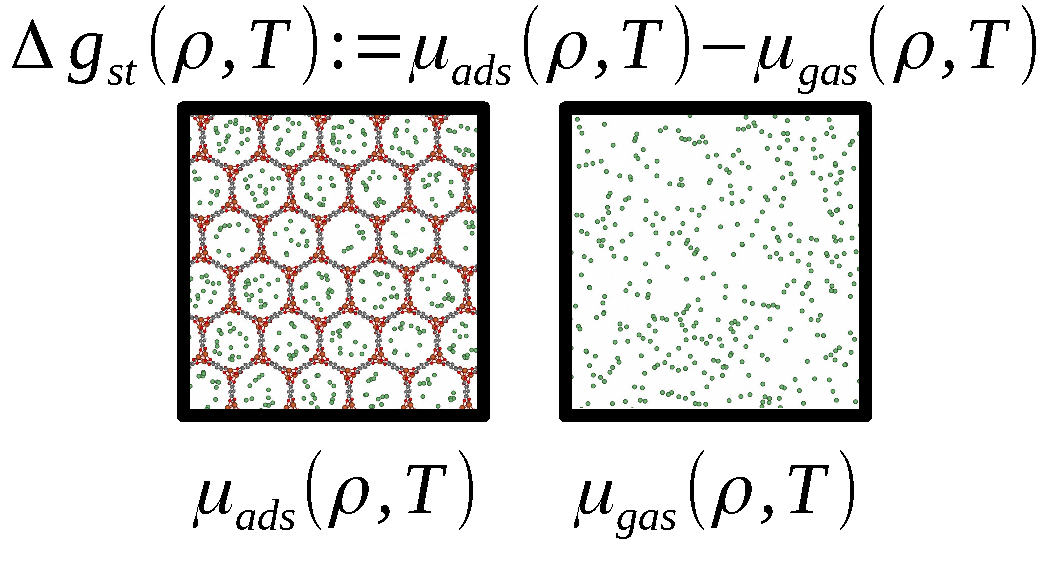
\includegraphics[width=\columnwidth]{g_st_simple.pdf}
    \caption{Cartoon illustrating the definition of $\gst$. For a given adsorbent and gas, $\gst$=$\gst (\rho, T)$ is defined as the difference in chemical potential between the adsorbed gas system and bulk gas system when both exhibit the same density $\rho$ and temperature $T$.}
    \label{fig:delta-G-cartoon}
\end{figure}

The parameter describing our idealized substrate is $\V$, the spatially uniform
potential felt by a gas molecule adsorbed in the idealized substrate. A natural
question is how this potential relates to the properties of real substrates.
The effect of $\V$ in our model is to shift the chemical potential $\mu$ of the
gas (see Sec.~\ref{sec:V_shifts_chem_pot}). Because our ideal substrate shifts
the chemical potential of the gas molecules by providing a spatially uniform
potential energy field, the entropy of the gas in the ideal substrate is equal
to the entropy of the gas in its bulk state at the same density and
temperature. In contrast, a real substrate provides a non-spatially uniform
potential. Consequently, the entropy of the gas inside a real substrate is
\emph{not} equal to the entropy of the bulk gas at the same density and
temperature. Therefore, the parameter analogous to $\V$ in a real substrate
will involve both energy and entropy. The real-substrate analog of $\V$ is the
shift of molar Gibbs free energy provided by the substrate, specifically an
\emph{isosteric} (or constant-density) shift of the Gibbs free energy:

\begin{equation}
   \gst(\rho, T) \equiv
   %\frac{G_{\text{ads}}(\rho, T) - G_{\text{gas}}(\rho, T)}{N}\\
    \mu_{\text{ads}}(\rho, T) - \mu_{\text{gas}}(\rho, T).
  % \gst(\rho, T) &\equiv g_{\text{gas}}(\rho, T) - g_{\text{ads}}(\rho, T)
  \label{eq:g_st}
\end{equation}
The isosteric Gibbs free energy difference $\gst$ is the difference in molar
Gibbs free energy (equivalent to chemical potential) between the adsorbed gas system and
the bulk gas \emph{with the same density of gas molecules}. The quantity $\gst$
does \emph{not} correspond to a change in the molar Gibbs free energy as a
molecule is adsorbed, which is zero under conditions of coexistence. The
quantity $\gst$ in a real substrate is a direct analog to $\V$ in our ideal
substrate because it is the chemical potential shift needed to impose on the
bulk gas in coexistence with the real substrate to achieve the same density as
in the substrate (compare with eqn.~\ref{eq:xi_vs_xi0}).
Figure~\ref{fig:delta-G-cartoon} illustrates a hypothetical experiment to
measure $\gst$ via a piston with a removable partition that separates a volume
of free space from the same volume of substrate. Note that $\gst$ is a property
of both the substrate and the identity of the gas. Because real substrates
offer a \emph{non}-spatially uniform potential, $\gst(\rho, T)$ is a function
of $\rho$ and $T$, unlike our ideal, homogenous substrate where $\gst(\rho,
T)=\V$. Consequently, throughout this article, we show $\gst(\rho, T)$ for real
substrates at both conditions relevant to gas storage and delivery, $\pfull$
and $\pempty$.

In practice, we can readily compute $\gst(\rho, T)$ of a real gas/substrate
system from (i) the (experimental or simulated) equilibrium adsorption isotherm
of the gas in the substrate and (ii) the (experimental or simulated) chemical
potential of the bulk gas. Consider the real substrate in thermodynamic
equilibrium with a bulk gas at fixed temperature $T$ and pressure $p$, and let
$\rho=\rho(p, T)$ be the density of gas in the substrate. At coexistence, the
chemical potential of the bulk gas is equal to the chemical potential of the
adsorbed gas in the substrate. Thus, we can use the experimentally known molar
Gibbs free energy of the pure, bulk gas system at temperature $T$ and pressure
$p$ to determine the molar Gibbs free energy of the adsorbed system:
$\mu_{\text{ads}}(\rho, T)=\mu_{\text{gas}}(p, T)$. We can then also look up
the known chemical potential of the bulk gas at the same density and
temperature as in the substrate, $\mu_{\text{gas}}(\rho, T)$. Via
eqn.~\ref{eq:g_st}, $\gst$ follows from subtracting the two quantities.

An interesting question is how $\gst$ relates to the commonly measured and
reported isosteric heat of adsorption $q_{st}$, which is roughly the energy
change when a gas molecule is adsorbed~\cite{sircar1999isosteric,
tian2017differential}. Figure~\ref{fig:qst-vs-delta-G} shows how $q_{st}$
compares to $\gst$ for several prominent adsorbents. In every case,
$|q_{st}|>|\gst|$ because the gas in the adsorbent always has less entropy than
the gas in the bulk at the same density and temperature. That is, while
adsorption is energetically favored, it is entropically disfavored due to the
restrictions imposed on the configuration of the gas molecules via steric
interactions with the substrate itself; this counters the energetic attraction.

\begin{figure}
    \centering
    \includegraphics[width=0.95\columnwidth]{qst-vs-delta-G}
    \caption{Relationship between $\gst$ and the isosteric heat
      $q_{st}$ for several prominent adsorbents at room
      temperature (data from Ref.~\cite{mason2014evaluating, garcia2018benchmark}). The dots represent the properties of methane
      adsorption at 5.8~bar and 65~bar. The $+$'s represent the
      properties of hydrogen adsorption at 5~bar and
      100~bar.}
    \label{fig:qst-vs-delta-G}
\end{figure}

\begin{figure}
    \centering
    \includegraphics[width=0.95\columnwidth]{methane-298-gst}
    \caption{The density-dependence of $\gst$ of methane in several
      adsorbents (298\ K). Note that $\gst$ is monotonic in
      $\rho$. Data from
      Refs.~\cite{mason2014evaluating, furukawa2009storage}.
    }
    \label{fig:methane-gst}
\end{figure}

\begin{figure}
\centering
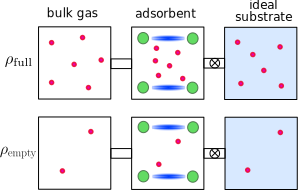
\includegraphics[width=0.95\columnwidth]{four-cases-pro}
\caption{A bulk gas reservoir is connected to a volume filled with adsorbent material (green/blue: material atoms, red: gas particles). The adsorbent is also connected, but with a closed valve, to an equal volume containing the ideal substrate (shaded blue background represents the uniform potential energy field $\V$) with an equal density of gas as in the adsorbent. The top (bottom) shows a realization of this connected system where the pressure of the bulk gas is $\pfull$ ($\pempty$), and thus the density of gas in the adsorbent is $\rhofull$ ($\rhoempty$) by definition. The deliverable capacity of the adsorbent is $\rhofull - \rhoempty$. We can determine if the deliverable capacity of gas in the ideal substrate is lower or higher than in the adsorbent by considering what happens when we open the valves connecting the two pairs of volumes containing adsorbent and the ideal substrate.}
\label{fig:delta-gst-maximum}
\end{figure}

\section{An upper bound when $\gst(\rho)$ is monotonic}\label{sec:monotonic}
Every adsorbent has a $\Delta g_\text{st}$ at $\pfull$ and $\pempty$ corresponding
to a full and empty density, $\rhofull$ and $\rhoempty$, respectively. The deliverable capacity of the adsorbent is equal to
the difference between the full and empty density. Examining
Fig.~\ref{fig:methane-gst}, we see that a significant variety of known
experimental $\Delta g_\text{st}$ curves are monotonic. Furthermore, our
qualitative argument in Section~\ref{sec:upper-bound} suggests that this
function \emph{should} monotonically increase for rigid substrates, as
increasing the density of gas causes some of the gas to reside in higher-energy
sites. If this is always the case, the deliverable capacity of a real material
(with a non-spatially uniform potential) with a given $\gst$ at $\pfull$ or
$\pempty$ is bounded below by the deliverable capacity in our idealized
substrate with $\V=\gst$, even for a value of $\V$ that is not optimal.

To show this, we perform a thought experiment illustrated in
Fig.~\ref{fig:delta-gst-maximum}. We begin with two pairs of volumes.  Two of
these volumes contain a real adsorbent material.  These adsorbent volumes are
connected to bulk gas reservoirs at $\pfull$ and $\pempty$ respectively, and
by definition contain gas at density $\rhofull$ and $\rhoempty$.  The other two volumes
volumes contain gas at a density equal to the two adsorbent volumes ($\rhofull$ and $\rhoempty$), but contain our
idealized substrate with uniform potential energy $\V$.

We now consider what happens if we open a diffusive connection between a
volume of adsorbent and a volume with an idealized substrate that initially contain
the same density of gas, for instance by connecting them with a tube. If the
chemical potential in the idealized substrate is higher than in the porous material,
then gas will flow out of the idealized substrate, lowering its density.  Conversely,
if the chemical potential is lower in the idealized substrate than in the
volume of porous material, then gas will flow into the idealized substrate, increasing
its density.
The difference in chemical potential between those two volumes is
\begin{align}
   \gst(\rho) - \V &= \left(\mu_{\text{ads}}(\rho) - \mu_{\text{gas}}(\rho)\right)
   - \left(\mu_{\V}(\rho) - \mu_{\text{gas}}(\rho)\right)
   \\
   &= \mu_{\text{ads}}(\rho) - \mu_{\V}(\rho).
\end{align}
where $\mu_{\text{ads}}(\rho)$ and $\mu_{\V}(\rho)$ are the chemical potentials
of gas in the porous material and ideal substrate with potential $\V$, respectively.
Thus if $\gst(\rhoempty) =
\V$, the low-density containers will remain at their initial density after
they are connected. Thus, the deliverable capacity of the adsorbent will be greater
than the deliverable capacity of the ideal substrate with uniform potential $\V$ if and
only if $\gst(\rhofull)<\V$, i.e. if $\gst(\rho)$ does \emph{not} monotonically
increase, since then the gas in the high-density system will flow from the ideal
substrate to the adsorbent. By the same token, if we consider the case where
$\gst(\rhofull) = \V$, then for the adsorbent to achieve a greater deliverable
capacity than the idealized substrate, the adsorbent must have less residual gas,
which means that gas must spontaneously flow from the low-density adsorbent to the
volume with potential $\V$, which means that $\gst(\rhoempty)>\V$. Once again,
exceeding our upper bound requires a material with a $\gst(\rho)$ that does not
increase monotonically.

Taken together, this indicates that not only is our absolute upper bound an
upper bound for rigid adsorbents, but the green curve labeled $\rho_D(\gst)$ in
Figs.~\ref{fig:methane-298-D}, \ref{fig:hydrogen-298-D}, and
\ref{fig:hydrogen-77-D} is an upper bound for materials with a non-optimal
$\gst$ at either $\pfull$ or $\pempty$.

\section{Cryogenic hydrogen storage}\label{sec:cryo-hydrogen}
One approach to increase the deliverable capacity is to reduce the storage
temperature. This is illustrated in Fig.~\ref{fig:hydrogen-77-D}, which shows
the upper bound to the deliverable capacity of hydrogen at 77\ K, the boiling
point of nitrogen. The DOE ULTIMATE target in this case looks far more
achievable, and with a much lower $|\gst|$. In fact, an empty tank at this
temperature can satisfy the DOE 2020 target. The DOE ULTIMATE target is 14\%
below the upper bound. Actual adsorbents fall far short of the theoretical maximum.

\begin{figure}
    \centering
    \includegraphics[width=0.95\columnwidth]{hydrogen-77-n-vs-G}
    \caption{Deliverable capacity of hydrogen at 77\ K as a function of the attractive Gibbs free energy $\gst$. Experimental deliverable capacities for several porous materials (data from Ref.~\cite{garcia2018benchmark}) are shown along with the experimental values for $\gst$ at the empty and full pressures shown as $+$'s connected by a line.}
    \label{fig:hydrogen-77-D}
\end{figure}
